\documentclass{article}

% if you need to pass options to natbib, use, e.g.:
%     \PassOptionsToPackage{numbers, compress}{natbib}
% before loading neurips_2021

% ready for submission
\usepackage[final]{neurips_2021}

% to compile a preprint version, e.g., for submission to arXiv, add add the
% [preprint] option:
%     \usepackage[preprint]{neurips_2021}

% to compile a camera-ready version, add the [final] option, e.g.:
%     \usepackage[final]{neurips_2021}

% to avoid loading the natbib package, add option nonatbib:
% \usepackage[nonatbib]{neurips_2021}
\bibliographystyle{abbrvnat}
\setcitestyle{authoryear,open={, },close={}} %Citation-related commands


\usepackage[utf8]{inputenc} % allow utf-8 input
\usepackage[T1]{fontenc}    % use 8-bit T1 fonts
\usepackage{hyperref}       % hyperlinks
\usepackage{url}            % simple URL typesetting
\usepackage{booktabs}       % professional-quality tables
\usepackage{amsfonts}       % blackboard math symbols
\usepackage{nicefrac}       % compact symbols for 1/2, etc.
\usepackage{microtype}      % microtypography
\usepackage{xcolor}         % colors
\usepackage{graphicx}
\usepackage{caption}
\usepackage{subcaption}
\captionsetup[table]{skip=10pt}
\usepackage{amsmath}
\usepackage[toc,page]{appendix}


% \usepackage{biblatex}
% \addbibresource{sample.bib} %Import the bibliography file


\title{A survey on generating private synthetic data}

% The \author macro works with any number of authors. There are two commands
% used to separate the names and addresses of multiple authors: \And and \AND.
%
% Using \And between authors leaves it to LaTeX to determine where to break the
% lines. Using \AND forces a line break at that point. So, if LaTeX puts 3 of 4
% authors names on the first line, and the last on the second line, try using
% \AND instead of \And before the third author name.

\author{
  Mahdi Alikhasi \\
  Department of Computing Science\\
  University of Alberta\\
  Edmonton, AB T6G 2R3 \\
  \texttt{alikhasi@ualberta.ca} \\
}

\begin{document}

\maketitle

\begin{abstract}
The goal of synthetic data generation is to create a database that matches the original ones in the sense of statistics. Nowadays, using machine learning tools became a trend to this end. One concern of these methods is that machine learning tools can compromise the privacy of individuals. In this project, we first survey existing techniques and then propose a new method.
\end{abstract}

\section{Introduction}

The wide range of datasets' usage in modern applications is undeniable. From a simple data analysis task to more complicated machine learning problems like speech recognition and image processing, we heavily rely on datasets more than ever. With the increasing amount of data and the trend of releasing datasets by companies, the concept of gathering and using this information brings a lot of concern about privacy because these datasets usually contain individuals' sensitive data, especially in the fields like medical diagnoses or genomics.

The problem of users' privacy has been studied from those early works on anonymization and differential privacy (\cite{dwork2011firm}). More formally, having a differentially private algorithm gives individuals the ability to denial. The idea here is that removing one row of data would not change the output of a query much, and the effect of each individual is neglectable, which gives them the ability to deny their presence in the database (\cite{ullman2011pcps}).

However, providing the privacy of a query on a dataset has its limitations, and it is not enough. To name a few, we have to change our software and analytical tools in order to work with differential privacy methods like the Laplacian mechanism (\cite{dwork2006calibrating}), which is an interactive algorithm. Moreover, sometimes it is necessary to have access to the whole database. One such scenario is when two companies want to collaborate and share data to improve accuracy. In these situations, it is more suitable to have access to the dataset instead of querying it. The problem of having access to the dataset while preserving the differential privacy can be addressed by generating a synthesized dataset from the original one in a private manner (\cite{ullman2011pcps}).

In this project, first, we compare the existing state-of-the-art methods with each other. This comparison is necessary since it gives us an insight into different approaches, their empirical quality in various tasks, and their limitation. In the next step, we propose a new framework for generating synthetic datasets in a differentially private approach that can both address the issue of privacy of individuals and have a good quality, which makes it suitable to be used as a training set in other machine learning tasks. The main goal here is that the proposed model should at first be private, and secondly, it should be able to create a synthesized dataset with similar statistical properties to the original dataset.


\section{Motivation}

Machine learning approaches, especially deep learning, have shown good results in recent years. However, these methods usually suffer from the need for large datasets to train. The first impact of being able to generate a synthetic dataset privately is that we could use this unlimited trope of synthetic data to train our model without being worried about problems like privacy. Besides, it enables us to share our datasets without privacy concerts.

The advantages and the perks of having a private synthetic dataset are even more. It will create an extra layer of privacy-preserving against the adversaries. It means that, if we use the private synthetic data to train a model in order to solve some problem; even if the adversary has access to the model or training dataset (which is the synthetic dataset here), the adversary can not infer any sensitive information about individuals from it (\cite{chen2018differentially}). More generally, we can show that any learning model trained on the private synthetic dataset is also differentially private (\cite{chen2018differentially}).


\section{Related Works}

One of the first works on the generation of synthetic data was the work of \cite{barak2007privacy}. In this work, the main focus was that the synthesized data should have the same statistical properties as the original. To satisfy it, the authors presented a non-polynomial time algorithm for creating a new database with the same two-way margin property while preserving differential privacy. Moreover, the work of \cite{ullman2011pcps} has shown that there is no polynomial-time algorithm to create a two-way margin synthesized private data. The limitation here is that the two-way margin property is not sufficient in complicated datasets like images.

With the emergence of machine learning, another trend has been created. Instead of preserving the statistical properties of the dataset using a holistic algorithm, we assume that there is an underlying distribution from which the original dataset was sampled. Then using machine learning, we aim to learn and approximate this underlying distribution. Finally, sampling from this learned underlying distribution will create new samples with the same statistical properties as the original one for us, which we can use as a synthetic dataset. This approach of learning the probabilistic model and statistical properties of the original dataset under privacy has been studied in the last decade ( \cite{zhang2016privtree}, and \cite{zhang2017privbayes}). Moreover, we can use deep learning to learn a more accurate presentation of the underlying distribution. This approach and its methodology have been shown in the works of \cite{xie2018differentially}, and \cite{jordon2018pate}. Both these works used generative adversarial networks, also known as GAN, as their generative models. The difference here is that in the former one, they used the DP-SGD method (\cite{abadi2016deep}), and in the latter, they used the PATE framework (\cite{papernot2016semi}) to preserve privacy. Furthermore, there are more generative models besides GANs. There is also the work of \cite{chen2018differentially} which uses two private deep networks side by side. One autoencoder and one variational autoencoder as a generator. Additionally, there is the work of \cite{takahashi2020differentially} which again uses the DP-SGD (\cite{abadi2016deep}) to train an autoencoder as a data generator.

One gap here among all the mentioned methods is that there is no work comparing these methods. Moreover, most of these methods show their utility and quality through visualization and the quality of synthesized data on image datasets like MNIST. In this project, we compare these methods both visually and theoretically. To compare methods visually, we consider a case of an image dataset when the goal is that the synthesized dataset has visual similarities. On the other hand, for the case of theoretical comparison, we analyze statistical similarities of the synthesized and original datasets with each other.

Furthermore, methods that use DP-SGD, including DP-GAN, require a large privacy budget to preserve privacy while their final results have poor quality. It motivates us in this project to use a private prediction or a noisy private sampling instead of making the learning algorithm private. To address it, we propose a new framework using variational autoencoder and noisy sampling in the following sections.


\section{Proposed Solution and Methodology}

Since the project aims to provide a solution for the private synthesize data generation, it is logical to start by comparing different existing state-of-the-art methods with each other, which is somehow absent in the previous studies. To compare these methods, we first try to see the results visually. The thing here is that although privacy is crucial, the main goal here is that the generated synthesized dataset has good quality, and it is easier to see the quality of different methods visually. For this part, we use the MNIST dataset as our original dataset and learn models on it. Moreover, to make the conditions fair, we choose an upper bound for the privacy budget. Then, after training the models on the MNIST dataset, we demonstrate the quality of models' output through random sampling from the generated synthesized dataset.

After visualizing the output of various frameworks, we can get a hunch on which method could be more accurate in real data. The next step is to understand whether the synthesized dataset is similar to the original one or not. For doing so, we need a measure that takes the whole dataset, and not limited to the individuals' information, into consideration and computes similarity. Thus, we use the method provided by the work of \cite{snoke2018pmse}. In the mentioned paper, the authors claim that a synthesized dataset has good quality if an arbitrary classification algorithm can not distinguish between the samples from the original one and the synthesized one. According to their work, we first generate a synthesized dataset. Then we train a classifier on half of the synthesized dataset and half of the original dataset. The labels for samples in the synthesized dataset will be one, and the label for the original samples will be zero. Using the pMSE metric (\cite{snoke2018pmse}), we will have:
\[
pMSE = \frac{1}{N} \sum_{i=1}^{N}(p_i - 0.5)^2
\]
Where $p_i$ is the classification's prediction for data $i$ in the test dataset. Here, the test dataset will be the other half of the synthesized dataset and the other half of the original dataset that we did not use during training.

The idea here is that if the classifier can not distinguish between the synthesized dataset and the original dataset on the test set, then $p_i$ would be near to $0.5$, which is a random choice. Thus, by calculating a mean square error on $p_i$ we can see that on average, how far is our prediction from random choice, 0.5. The lesser pMSE is, the more similar the synthesized dataset and original dataset are, and that means the classifier can not distinguish between them. By this means, we can compare different methods of generating synthesized data and their quality.

Although pMSE will provide us with a metric for comparison, it will not provide us with an explanation of the results. It can be done by constructing a distance metric and studying the parameters and factors that affect this distance separately. For finding the distance between the synthesized dataset and the original one, first, we calculate the correlation matrix of the features in the original dataset and the synthesized one alongside the momentum of each feature. Then, by comparing the correlation matrix of the synthesized dataset and the original one, we can specify whether the relation between features is preserved or not. What is more, by comparing the momentums it is possible to highlight the similarities in each feature between the synthesized dataset and the original one in a stand-alone manner.  We introduce a distance measurement to compare different methods, which is the weighted sum of distances of different momentums and correlation matrix. The less this distance measure is, the more realistic and similar the synthetic dataset is. For categorical features, comparison of the plot and the relative proportion of features' categories are sufficient. To this end, the Census Adult dataset will be used, and we analyze models and synthesized datasets on this dataset. The dataset is selected from the OpenML library \footnote{The dataset that we used can be found at https://www.openml.org/d/1119}.

All these metrics studied so far are associated with the quality of the synthesized data. However, another crucial part of our approach is privacy. To have an insight into the privacy of these models, we take into consideration the nearest neighbor of each synthesized sample in the original dataset. Our methodology here is that for each sample in the synthesized dataset first, we find the nearest individual in the original dataset. Then we calculate the euclidean distance between these two. By calculating the distance for all samples in the synthesized dataset, it ables us to study the variance and the mean of this distance. The intuition here is that for being private, all the samples should have a similar effect on the data generation of the synthesized dataset. This idea is very close to the motivation behind the clipping part of DP-SGD (\cite{abadi2016deep}). It can be interpreted that the variance of the distance between each sample in the synthesized dataset and its nearest match in the original one should be as low as possible. In addition, we prefer that the generative model does not overfit the samples in the original dataset. It can be seen as the mean distance between samples in the synthesized dataset and their corresponding match in the original one. Thus, we prefer to have a high mean distance. Another study here is to estimate the gap between the nearest match of samples and the second nearest match.

Finally, we propose a new framework for private synthetic data generation. Here, our approach is very similar to the PATE (\cite{papernot2016semi}). In this paper, to address the limitations of methods like DP-SGD (\cite{abadi2016deep}), the authors came up with a teacher-student model which uses an ensemble model as a teacher. Moreover, they use noisy voting to provide privacy. Since the teacher models are not private themself, privacy will be compromised if an adversary has access to the models. They used a student model which will train on the output of the teacher part. Their work is based on having a private way of prediction, contracting with DP-SGD that makes the learning algorithm private. Similarly, our proposed method is based on making the sampling of data generation private. The intuition here is similar to the one in PATE.

Our strategy here is to divide the dataset into several sub-datasets and train a generative model on each of these sub-datasets separately. After the training phase, we can use these models to generate new samples, which can be done using a sample selection block. Here, at each timestep, all the generative models will generate new samples, and the sample selection block will choose one of them. Through repeating this procedure $n$ times, we can obtain an intermediate synthesized dataset. The details of the sample selection block will be described further. This structure is much similar to the method known as ensemble learning (\cite{dietterich2000ensemble}). The difference is that in ensemble learning, a weighted voting approach is used to aggregate the results of each model, while our structure has a sample selection block.

The only structure here left to discuss is the sample selection block. This block inputs a series of samples alongside the training dataset, and selects one of the input samples, and returns it as an output. To do so, for each sample it finds the closest match, using Euclidean distance, in the training dataset. After that, it will add a Laplacian noise to this calculated distance to compute a noisy distance. It chooses the one with the largest noisy distance value among all samples. Our intuition here is that if there is an outlier in the training dataset, the generator can get overfit on it to increase the accuracy, while this can compromise privacy. In this case, the distance between that individual and a synthesized sample is low, and the sample selection block will not choose it with a high probability because of its structure. Generally speaking, if a synthesized sample gets very close to a match in the original one, its noisy distance is low, and the sample selection block will not choose it. On the other hand, because of the noise added here, there is a kind of uncertainty about selecting a sample that would guarantee privacy.

\begin{figure}[htp]
    \centering
    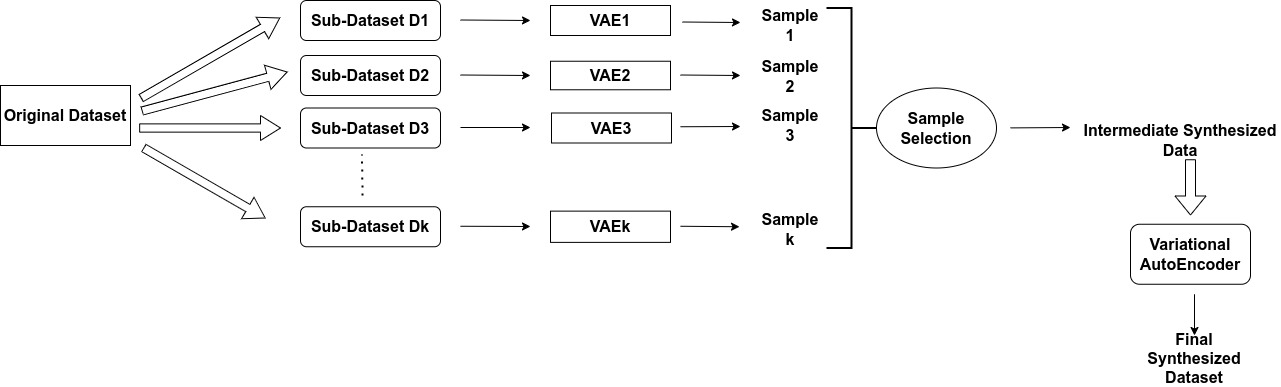
\includegraphics[width=1\textwidth]{images/framework.jpg}
    \caption{Proposed framework: (1) an ensemble of generative models trained on subsets of the original dataset. (2) each model outputs a sample after training. (3) sample selection block selects one of the samples to create the intermediate dataset. (4) Final student model trains on the intermediate dataset. Note that we use variational autoencoder models as our generator.}
    \label{fig:framework}
\end{figure}

Figure \ref{fig:framework} shows the structure of our proposed framework.


\section{Results}

Our strategy toward studying the statistical similarity of the original dataset and the synthesized one starts by computing the correlation matrix of features. As discussed earlier, this will provide us with the relation between features in the original dataset and the synthesized one. For this section, we run our experiments on the Census Adult dataset. We used the implementation provided here\footnote{https://github.com/BorealisAI/private-data-generation}, and here\footnote{https://github.com/vanderschaarlab/mlforhealthlabpub/tree/main/alg/pategan} to generate synthesized data on the Census Adult dataset. Then, after generating it, we compared the results\footnote{For the DP-GAN implementation, we used the variant that uses Wasserstein distance. This variant is also known as DP-WGAN.}. To make the learning faster, we normalized the Census Adult dataset features to be in the range of [0, 1], and after generating synthesized data we reversed the normalization. What is more, for the implementation of our proposed method we used 10 variational autoencoders. The details of this implementation are provided in appendix A.

\begin{figure}
     \centering
     \begin{subfigure}[b]{0.48\textwidth}
         \centering
         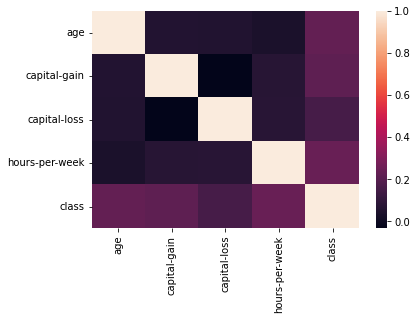
\includegraphics[width=\textwidth]{images/census_heatmap_original.png}
         \caption{Original Dataset}
         \label{fig:corrmatrix_original}
     \end{subfigure}
     \hfill
     \begin{subfigure}[b]{0.48\textwidth}
         \centering
         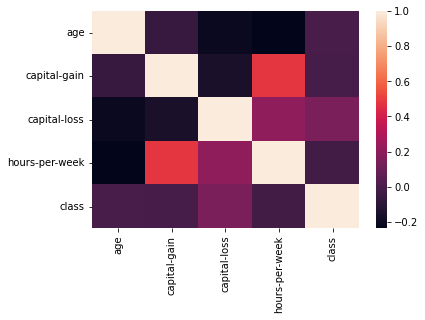
\includegraphics[width=\textwidth]{images/census_heatmap_dpgan.png}
         \caption{DP-WGAN Output}
         \label{fig:corrmatrix_dpgan}
     \end{subfigure}
     
     \bigskip
     \begin{subfigure}[b]{0.48\textwidth}
        \centering
        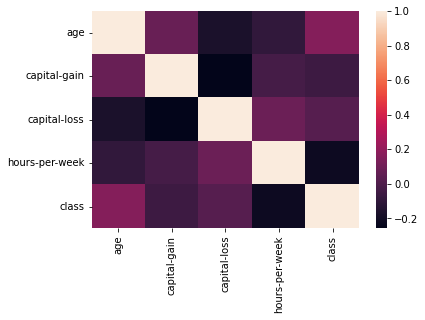
\includegraphics[width=\textwidth]{images/census_heatmap_pategan.png}
        \caption{PATE-GAN Output}
        \label{fig:corrmatrix_pategan}
    \end{subfigure}
    \hfill
     \begin{subfigure}[b]{0.48\textwidth}
         \centering
         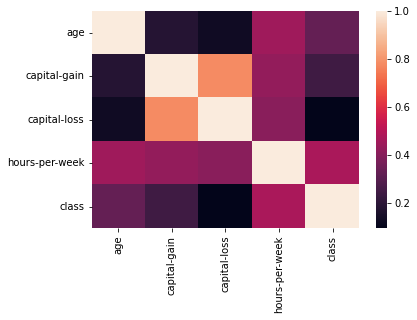
\includegraphics[width=\textwidth]{images/census_heatmap_teacher.png}
         \caption{Proposed Model Output}
         \label{fig:corrmatrix_teacher}
     \end{subfigure}
        \caption{Heatmap of Correlation matrix}
        \label{fig:heatmap}
\end{figure}

Figure \ref{fig:heatmap} shows the heatmap of feature correlation in the original dataset. This figure gives us intuition that to some extent all of the provided algorithms preserve the relations between features. To experiment in more details, we calculate the sum square error of the correlation matrix as follow:
\[ SSE = \sum{(MC - OC) ^ 2} \]
Where $MC$ is the correlation matrix of the model under study, and $OC$ is the correlation matrix of the main dataset. The power operator is element-wise power in a matrix, and the sum is the sum over all elements of each row in a matrix. Results are shown in the table \ref{table:correlation_matrix}.

\begin{table}[ht]
    \centering
    \begin{tabular}{||c | c c c||}
        \hline
        & DP-WGAN & PATE-GAN & Proposed Model \\ [0.5ex] 
        \hline\hline
        age             & 0.206777          & \textbf{0.071572} & 0.199806 \\ 
        capital-gain    & 0.247967          & \textbf{0.135406} & 0.808232 \\
        capital-loss    & \textbf{0.096976} & 0.118604          & 0.783392 \\
        hours-per-week  & 0.328045          & \textbf{0.237578} & 0.458623 \\
        class           & 0.168672          & 0.307770          & \textbf{0.070163} \\ [1ex] 
        \hline
    \end{tabular}
    \caption{Sum of Square Error of correlation matrix between various approaches and original dataset.}
    \label{table:correlation_matrix}
\end{table}

In the table \ref{table:correlation_matrix}, the best method in each row is highlighted in bold. It can be interpreted from this table that PATE-GAN can mimic the relation between features more accurately. The main reason for this trend is that since DP-WGAN uses DP-SGD, the noises added to gradient descent will eventually accumulate on each other and affect the final accuracy. In this experiment, the privacy budget is set to be fixed to $\epsilon = 8$. Note that although Census Adult has only 14 features, most of its features are categorical, which makes the training even harder. Another interesting part here is that the Census Adult dataset is a classification task in which the labels are the 'class' feature. As you can see in the table, our proposed method was able to capture the correlation in this feature more accurately.

As we discussed earlier in the methodology section, the next step is to study the similarity of features in the synthesized dataset and the original dataset in a stand-alone manner. To do so, we compute the mean and variance of each feature.
           
\begin{table}[ht]
    \centering
    \begin{tabular}{||c |c c c c||}
        \hline
        & Original Dataset & DP-WGAN & PATE-GAN & Proposed Model \\ [0.5ex] 
        \hline\hline
        age             & 38.5326   & 1.7792            & 44.472145     & \textbf{37.5152} \\ 
        capital-gain    & 1033.6284 & 11579.4356        & 50058.197550  & \textbf{8187.5314} \\
        capital-loss    & 93.6952   & -499.8672         & 2191.371395   & \textbf{298.2812} \\
        hours-per-week  & 40.5150   & -8.5138           & 49.421968     & \textbf{40.5828} \\
        class           & 0.2442    & \textbf{0.2514}   & 0.500198      & 0.3610 \\ [1ex] 
        \hline
    \end{tabular}
    \caption{Mean value of each feature in original and synthesized datasets.}
    \label{table:mean}
\end{table}

\begin{table}[ht]
    \centering
    \begin{tabular}{||c |c c c c||}
        \hline
        & Original Dataset & DP-WGAN & PATE-GAN & Proposed Model \\ [0.5ex] 
        \hline\hline
        age             & 1.842814e+02  & 1.062483e+03  & \textbf{2.101505e+02} & 9.927242e+01 \\ 
        capital-gain    & 4.972772e+07  & 1.481932e+09  & \textbf{2.485816e+08} & 2.732494e+08 \\
        capital-loss    & 1.687529e+05  & 1.856199e+06  & 4.581812e+05      & \textbf{2.453345e+05} \\
        hours-per-week  & 1.465983e+02  & 1.357706e+03  & 3.388614e+02      & \textbf{5.432961e+01} \\
        class           & 1.846033e-01  & \textbf{1.882357e-01}  & 2.500988e-01      & 2.307251e-01 \\ [1ex] 
        \hline
    \end{tabular}
    \caption{Variance value of each feature in original and synthesized datasets.}
    \label{table:variance}
\end{table}

Table \ref{table:mean} and table \ref{table:variance} show the first two momentum of data. It is more suitable that the momentums be as close as possible to the original ones. The closest values are highlighted in bold. The results show that our proposed method could preserve the statistical properties of the original dataset more accurately in terms of momentum. It is worth mentioning that the results from PATE-GAN are very close to the original dataset too, which shows this method can work on this dataset quite well. Another interesting part is that DP-GAN is not much successful in synthesizing datasets. Our hunch is that it can be mainly because of two reasons. First, the Census Adult dataset is mostly categorical. It has 14 features, but after doing one hot encoding, the number of features will increase to 98. In this situation, our training set is sparse, which can adversely affect the training of this model. Another reason can be that the maximum privacy budget here is not enough for this method to capture the complexity of the training dataset. Both of these intuitions need further experiments.

Moving next to categorical features, we analyze the histogram of them in Figure \ref{fig:histogram}. Results indicate that our model was able to mimic the trend in the categorical data better than the other two methods.

\begin{figure}
     \centering
     \begin{subfigure}[b]{0.24\textwidth}
         \centering
         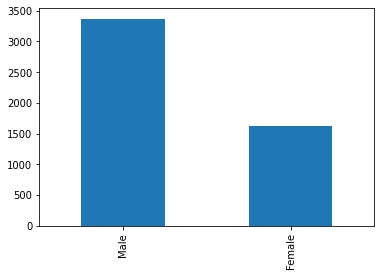
\includegraphics[width=\textwidth]{images/original_hist_sex.png}
         \caption{Original Dataset}
         \label{fig:histogram_original}
     \end{subfigure}
     \hfill
     \begin{subfigure}[b]{0.24\textwidth}
         \centering
         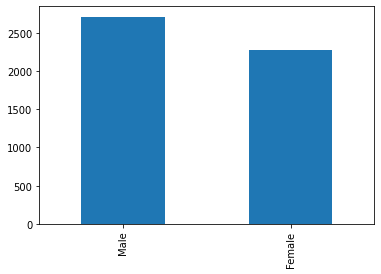
\includegraphics[width=\textwidth]{images/dpgan_hist_sex.png}
         \caption{DP-WGAN Output}
         \label{fig:histogram_dpgan}
     \end{subfigure}
     \hfill
     \begin{subfigure}[b]{0.24\textwidth}
        \centering
        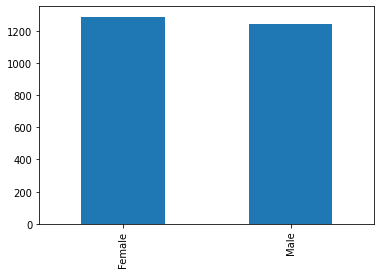
\includegraphics[width=\textwidth]{images/pategan_hist_sex.png}
        \caption{PATE-GAN Output}
        \label{fig:histogram_pategan}
    \end{subfigure}
    \hfill
     \begin{subfigure}[b]{0.24\textwidth}
         \centering
         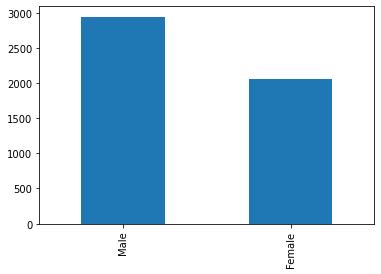
\includegraphics[width=\textwidth]{images/teacehr_hist_sex.png}
         \caption{Our Output}
         \label{fig:histogram_teacher}
     \end{subfigure}
        \caption{Histogram of sex feature}
        \label{fig:histogram}
\end{figure}

So far, we analyzed datasets using different matrices and various perspectives. The final question here is how to consider all these metrics together. To find the quality of a synthesized dataset here, we introduce a distance metric that uses all the previous analyzes. It is as equation \ref{eq:distance}.
\begin{multline}
Distance = \sum SSE + \sum_{features}(model\;mean - original\;dataset\;mean)^2 \\
+ \sum_{features}(model\;variance - original\;dataset\;variance)^2 \\
+ \sum_{features}(\sum_{category}(model\;count - original\;dataset\;count)^2)
\label{eq:distance}
\end{multline}


For more accurate results, we normalized this distance to get equation \ref{eq:distance_normalize}, where w is some weight. The results for equation \ref{eq:distance_normalize} are shown in table \ref{table:distance}.

\begin{multline}
Distance = w_1 * \sum SSE + w_2 * \sum_{features}(1 - \frac{model\;mean}{original\;dataset\;mean})^2 \\
+ w_3 * \sum_{features}(1 - \frac{model\;variance}{original\;dataset\;variance})^2 \\
+ \sum_{features}w_{4i} * (\sum_{category}(1 - \frac{model\;count}{original\;dataset\;count})^2)
\label{eq:distance_normalize}
\end{multline}

\begin{table}[ht]
    \centering
    \begin{tabular}{||c c c||}
        \hline
        DP-WGAN & PATE-GAN & Proposed Model \\ [0.5ex] 
        \hline\hline
        236.1874 & 137.8452 & \textbf{5.9794} \\ [1ex] 
        \hline
    \end{tabular}
    \caption{Distance of the synthesized dataset from the original one.}
    \label{table:distance}
\end{table}

This result is one of the most crucial parts of our project. The reason that the distance for PATE-GAN and DP-GAN is high is that these methods have trouble synthesizing categorical data. It can be seen in the histograms too. The high difference between the histograms of categorical data leads to this high distance. It also indicates that one aspect of improvement for these methods is to make them more suitable for sparse datasets like categorical ones, which can lead us to some future works.

Our final step toward this project is to study the pMSE. As we mentioned earlier, it shows that to what extent the synthesized data can not be distinguished by a classifier. Thus, it is a good metric to be considered as the quality of the synthesized dataset. Table \ref{table:pmse} shows the results.

\begin{table}[ht]
    \centering
    \begin{tabular}{||c c c||}
        \hline
        DP-WGAN & PATE-GAN & Proposed Model \\ [0.5ex] 
        \hline\hline
        0.2447 & 0.2083 & \textbf{8.2675e-05} \\ [1ex] 
        \hline
    \end{tabular}
    \caption{pMSE of the synthesized dataset created by different methods.}
    \label{table:pmse}
\end{table}

In this section, an SVM classifier is used for classification. To this end, we used sklearn library\footnote{https://scikit-learn.org/} with a linear kernel. It indicates that although the data synthesized by PATE-GAN have statistical similarities to the original one, a classifier is still able to distinguish it from the original dataset. Moreover, this data gives us more important outcomes. First, with the same amount of privacy, PATE-GAN leads to better-synthesized data compared to DP-GAN. In other words, DP-GAN requires a higher privacy budget for satisfactory outputs. Secondly, both DP-GAN and PATE-GAN have trouble synthesizing categorical features and sparse datasets. Third, our motivation in the first place was the quality of the synthesized dataset. It can be seen that PATE-GAN is still far from this requirement in our empirical study. 


\section{Conclusion}
The most important result of this survey would be to present a new perspective on studying synthesized datasets. We analyzed a dataset from different aspects and using pMSE we showed that having similar statistics can not be enough, and a classifier is still able to distinguish synthesized data. It is worth mentioning that through our experiments, with the same amount of privacy budget, PATE-GAN showed better results compared to DP-GAN.

Moreover, we showed that the mentioned methods have trouble synthesizing sparse datasets. One future work can be to improve our learning algorithms and frameworks against these kinds of datasets.

We introduced a distance metric, which gives us a foundation for analyzing the quality of a synthesized dataset. Since this metric determines how far two databases are from each other, one way of improving our learning algorithm in future works can be using this metric as some feedback to improve outputs.

Finally, we introduced a new framework that uses the intuition from the PATE framework to do a noisy sampling, and we showed its utility compared to other methods. It is still left to be discussed in further detail the perks and disadvantages of this framework, which can be done in future works.
\newpage
\noindent
\bibliography{sample}

\newpage
\noindent
\begin{appendices}
\section{Network Setting}
To implement our proposed model, we used the TensorFlow library. Our Model consists of 10 generators and a sample selection block. Each of these generators is a variational autoencoder.
The details of each variational autoencoder are as follows:
In the encoder part, there is one hidden layer with Relu activation. This layer consists of 64 nodes.
The latent space layer, z, consists of 4 nodes.
The decoder part consists of one hidden layer with a Relu activation function and 64 nodes. The final layer is an output layer with the shape same as the input layer.
\end{appendices}

\end{document}